\documentclass{beamer}
\usetheme{Madrid}
\usecolortheme{default}
\usepackage{tikz}
\usepackage{amsmath}
\usepackage{booktabs}
\usepackage{graphicx} % Required for including images

\title{Models, Idealizations, and Abstraction}
\subtitle{Tools for Good Thinking}
\author{Brendan Shea, PhD}
\date{Intro to Logic}



\begin{document}
	
	\frame{\titlepage}
	
	\begin{frame}{What is a Model? Understanding Simplified Representations}
		\begin{itemize}
			\item A \textbf{model} is a simplified version of something complex that helps us understand, predict, or explain how things work.
			\item Models intentionally leave out certain details to focus on what matters most for a specific purpose.
			\item We use models every day without realizing it—from toy cars to mental pictures of how our friends might react to news.
			\item The key insight is that all models are "wrong" in some way because they're simpler than reality, but many are still incredibly useful.
		\end{itemize}
		
		\begin{block}{Remember}
			A model's value comes not from being perfect, but from being useful for its intended purpose.
		\end{block}
	\end{frame}
	
	\begin{frame}{Why We Need Models: Making Complex Things Understandable}
		\begin{itemize}
			\item The real world contains far too much information for our brains to process all at once.
			\item Models act as \textbf{cognitive tools} that reduce this overwhelming complexity to manageable chunks we can work with.
			\item Without models, we couldn't make predictions, plan for the future, or communicate complex ideas to others.
			\item Scientists, engineers, teachers, and even artists all rely on models to do their work effectively.
		\end{itemize}
		
		\begin{example}
			When giving directions to your house, you don't describe every tree and crack in the sidewalk—you create a simple model using major landmarks and street names.
		\end{example}
	\end{frame}
	
	\begin{frame}{Abstraction: The Art of Leaving Things Out}
		\begin{itemize}
			\item \textbf{Abstraction} is the process of removing specific details to reveal general patterns or essential features.
			\item When we abstract, we deliberately ignore certain aspects of reality to highlight others that matter more for our purposes.
			\item Good abstraction requires judgment about what to keep and what to discard—this is a skill that improves with practice.
			\item The same real-world situation can be abstracted in different ways depending on what we're trying to understand or accomplish.
		\end{itemize}
		
		\begin{alertblock}{Warning}
			Too much abstraction makes a model useless; too little makes it too complicated to work with.
		\end{alertblock}
	\end{frame}
	
	\begin{frame}{Idealization: When Perfect Spheres Don't Exist}
		\begin{itemize}
			\item \textbf{Idealization} is a special type of abstraction where we imagine perfect or extreme versions of things that don't exist in reality.
			\item Physics teachers talk about "frictionless surfaces" and "perfect vacuums"—these idealizations help us understand fundamental principles.
			\item In everyday life, we idealize when we think about "the perfect friend" or "an absolutely fair game."
			\item Idealizations are powerful because they show us limiting cases and help us understand what happens when certain factors are pushed to extremes.
		\end{itemize}
		
		\begin{center}
			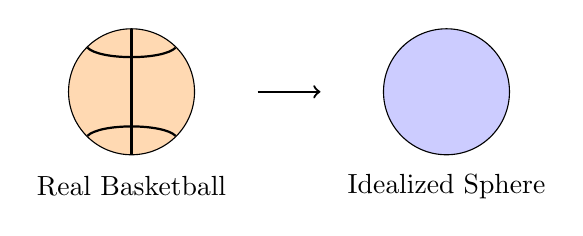
\begin{tikzpicture}[scale=0.8]
				% Real basketball
				\draw[fill=orange!30] (0,0) circle (1cm);
				\node at (0,-1.5) {Real Basketball};
				\draw[thick] (-0.7,0.7) .. controls (-0.5,0.5) and (0.5,0.5) .. (0.7,0.7);
				\draw[thick] (-0.7,-0.7) .. controls (-0.5,-0.5) and (0.5,-0.5) .. (0.7,-0.7);
				\draw[thick] (0,-1) -- (0,1);
				
				% Arrow
				\draw[->, thick] (2,0) -- (3,0);
				
				% Perfect sphere
				\draw[fill=blue!20] (5,0) circle (1cm);
				\node at (5,-1.5) {Idealized Sphere};
			\end{tikzpicture}
		\end{center}
	\end{frame}
	\begin{frame}{Maps as Models: Why Your GPS Doesn't Show Every Blade of Grass}
		\begin{itemize}
			\item Maps are perfect examples of models because they represent three-dimensional space on a two-dimensional surface.
			\item Every map involves \textbf{selective representation}—showing roads but not individual houses, or showing countries but not cities.
			\item The level of detail in a map depends on its purpose: a hiking map shows elevation changes, while a subway map ignores them completely.
			\item Your GPS map updates in real-time but still leaves out countless details like the color of buildings or the number of windows.
		\end{itemize}
		
		\begin{table}
			\centering
			\begin{tabular}{lcc}
				\toprule
				Map Type & Shows & Ignores \\
				\midrule
				Road Map & Streets, highways & Building heights \\
				Topographic & Elevation, terrain & Traffic patterns \\
				Political & Borders, capitals & Physical features \\
				Weather & Temperature, precipitation & Street names \\
				\bottomrule
			\end{tabular}
		\end{table}
	\end{frame}
	
	\begin{frame}{The Subway Map Example: When Distortion Helps}
		\begin{itemize}
			\item The famous London Underground map \textbf{deliberately distorts} geographic reality to make the system easier to navigate.
			\item Stations are evenly spaced on the map even though they're not in real life, and the Thames River is simplified to a few straight lines.
			\item This "wrong" map is more useful than a geographically accurate one because it optimizes for its purpose: helping people navigate between stations.
			\item The map's designer, Harry Beck, realized that subway riders care about connections and sequence, not precise distances or directions.
		\end{itemize}
		
		\begin{block}{Design Principle}
			The best model isn't the most accurate one—it's the one that best serves its intended users and purpose.
		\end{block}
	\end{frame}
	
	
	\begin{frame}
		\frametitle{London Underground Map}
		\begin{figure}
			\centering
			% space for the caption or other content.
			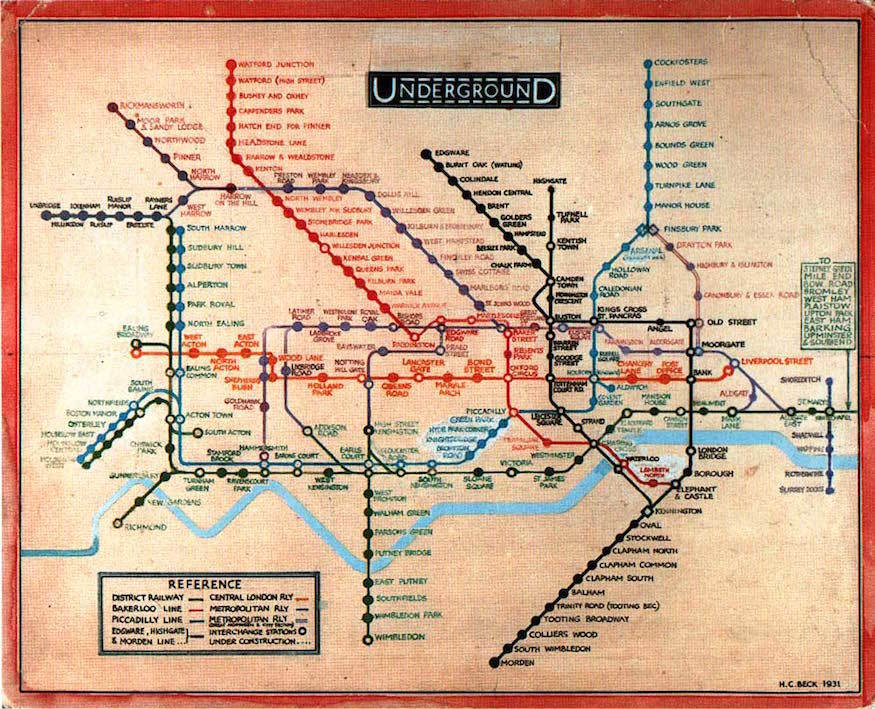
\includegraphics[width=\textwidth, height=0.8\textheight, keepaspectratio]{images/lu_map_1931.jpg}
			\small
			\caption{The 1931 map that changed the way subway maps were drawn.}
		\end{figure}
	\end{frame}
	
	
	
	\begin{frame}{Scale Models: From Toy Planes to Architectural Blueprints}
		\begin{itemize}
			\item \textbf{Scale models} maintain proportional relationships while changing size, allowing us to work with things too large or small to handle directly.
			\item Architects build small models of buildings to test designs, while engineers use scaled-up models of tiny components to understand how they work.
			\item The key to scale models is maintaining \textbf{relevant proportions}—a 1:100 model means every dimension is exactly 100 times smaller.
			\item Some properties scale perfectly (like shape), while others don't (like material strength), which is why we must be careful when interpreting scale models.
		\end{itemize}
		
		\begin{example}
			\begin{itemize}
				\item Model airplane: Tests aerodynamics at 1:50 scale
				\item Architectural model: Shows building appearance at 1:200 scale
				\item Molecular model: Enlarges atoms billions of times for visibility
				\item Solar system model: Shrinks vast distances to fit in a classroom
			\end{itemize}
		\end{example}
	\end{frame}
	
	\begin{frame}{Mental Models: How We Think About Everyday Life}
		\begin{itemize}
			\item \textbf{Mental models} are the internal representations we use to understand how things work and predict what will happen.
			\item You have mental models for everything from how your friends will react to jokes to how long your homework will take.
			\item These models are built from experience and constantly updated—when surprised, we revise our mental models to be more accurate.
			\item We often don't realize we're using mental models until they fail us and we have to consciously think about why our expectations were wrong.
		\end{itemize}
		
		\begin{alertblock}{Common Mental Model Errors}
			\begin{itemize}
				\item Assuming everyone thinks like you do
				\item Oversimplifying complex situations
				\item Not updating models when given new information
				\item Applying models outside their useful range
			\end{itemize}
		\end{alertblock}
	\end{frame}
	
	\begin{frame}{The "Average Person" Model: Statistics and Simplification}
		\begin{itemize}
			\item The \textbf{statistical average} is a model that represents an entire group with a single number or set of characteristics.
			\item When we say "the average teenager needs 9 hours of sleep," we're creating a simplified model that ignores individual variation.
			\item This model is useful for making general predictions and policies, but it can be misleading if we forget that no real person is perfectly average.
			\item Statistical models help us see patterns in large groups that would be invisible if we tried to track every individual separately.
		\end{itemize}
		
		\begin{center}
			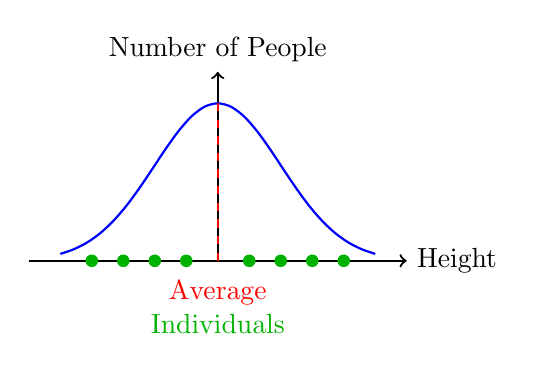
\begin{tikzpicture}[scale=0.8]
				% Draw normal distribution
				\draw[thick,->] (-3,0) -- (3,0) node[right] {Height};
				\draw[thick,->] (0,0) -- (0,3) node[above] {Number of People};
				% Bell curve
				\draw[thick,blue,domain=-2.5:2.5,smooth,variable=\x] plot ({\x},{2.5*exp(-\x*\x/2)});
				% Average line
				\draw[thick,red,dashed] (0,0) -- (0,2.5);
				\node[red] at (0,-0.5) {Average};
				% Individual points
				\foreach \x in {-2,-1.5,-1,-0.5,0.5,1,1.5,2}
				\fill[green!70!black] (\x,0) circle (0.1);
				\node[green!70!black] at (0,-1) {Individuals};
			\end{tikzpicture}
		\end{center}
	\end{frame}
	
	\begin{frame}{Weather Models: Predicting the Unpredictable}
		\begin{itemize}
			\item Weather models use \textbf{mathematical equations} to simulate how air pressure, temperature, and moisture interact in the atmosphere.
			\item These models divide the atmosphere into millions of 3D boxes and calculate how conditions in each box change over time.
			\item Even the best weather models lose accuracy after about 10 days because tiny measurement errors grow exponentially—this is called \textbf{chaos theory}.
			\item Meteorologists run multiple models with slightly different starting conditions to estimate the uncertainty in their predictions.
		\end{itemize}
		
		\begin{block}{Model Limitations}
			Weather models can predict general patterns (like storm systems) better than specific details (like exactly where rain will fall in your neighborhood).
		\end{block}
	\end{frame}
	
	\begin{frame}{Economic Models: Supply, Demand, and Reality}
		\begin{itemize}
			\item Economic models like \textbf{supply and demand curves} simplify the incredibly complex world of human buying and selling behavior.
			\item These models assume people are "rational actors" who always try to maximize their benefit, though real people often act emotionally or irrationally.
			\item The basic model ignores factors like advertising, social pressure, and habit, but it still helps predict how prices change when supply or demand shifts.
			\item Economists build more complex models by adding factors back in, but even these can't capture all the messiness of real human behavior.
		\end{itemize}
		
		\begin{example}
			\scriptsize
			Simple Supply and Demand Model Assumptions:
			\begin{itemize}
				\item Perfect information (everyone knows all prices)
				\item No transaction costs (buying is free and instant)
				\item Identical products (all apples are the same)
				\item Many buyers and sellers (no monopolies)
			\end{itemize}
		\end{example}
	\end{frame}
	
	\begin{frame}{The Atom Model: From Plum Pudding to Electron Clouds}
		\begin{itemize}
			\item Scientific models evolve as we gather new evidence—the model of the atom has changed dramatically over the past 200 years.
			\item Thomson's "plum pudding" model imagined electrons embedded in positive charge like raisins in pudding, but experiments proved this wrong.
			\item Bohr's model showed electrons in fixed orbits like planets, which explained some observations but failed to explain others.
			\item Today's \textbf{quantum mechanical model} describes electrons as probability clouds, which is harder to visualize but matches experimental results better.
		\end{itemize}
		
		\begin{table}
			\centering
			\small
			\begin{tabular}{lll}
				\toprule
				Model & Year & Key Feature \\
				\midrule
				Dalton & 1803 & Solid spheres \\
				Thomson & 1897 & Plum pudding \\
				Rutherford & 1911 & Nucleus + empty space \\
				Bohr & 1913 & Fixed electron orbits \\
				Quantum & 1926 & Probability clouds \\
				\bottomrule
			\end{tabular}
		\end{table}
	\end{frame}
	
	\begin{frame}{Sports Statistics: Modeling Athletic Performance}
		\begin{itemize}
			\item Sports use \textbf{statistical models} to reduce complex athletic performances to numbers that can be compared and analyzed.
			\item A basketball player's "shooting percentage" models their scoring ability with a single number, ignoring factors like defense pressure or game importance.
			\item Advanced models like "player efficiency rating" try to capture more aspects of performance, but they still can't measure intangibles like leadership or clutch performance.
			\item These models help coaches make decisions and fans understand the game, but overreliance on statistics can miss crucial human elements.
		\end{itemize}
		
		\begin{alertblock}{The Moneyball Revolution}
			Baseball's Oakland Athletics used statistical models to find undervalued players, proving that better models can provide competitive advantages even with limited resources.
		\end{alertblock}
	\end{frame}
	
	\begin{frame}{Social Media Algorithms: Models of Human Behavior}
		\begin{itemize}
			\item Social media platforms use \textbf{algorithmic models} to predict what content you'll find engaging based on your past behavior.
			\item These models track metrics like clicks, likes, viewing time, and shares to build a profile of your interests and preferences.
			\item The algorithm's model of you is constantly updating—every interaction teaches it more about what keeps you scrolling.
			\item These models are powerful but can create "filter bubbles" where you only see content that matches the algorithm's model of your interests.
		\end{itemize}
		
		\begin{block}{How the Model Sees You}
			\begin{center}
				You = Past Clicks + Time Spent + Similar Users + Trending Topics
			\end{center}
			This simplified equation can predict your behavior surprisingly well, but it reduces your complex personality to data points.
		\end{block}
	\end{frame}
	
	\begin{frame}{Video Game Physics: When Close Enough is Good Enough}
		\begin{itemize}
			\item Video games use \textbf{simplified physics models} that create believable movement without calculating every real-world force.
			\item Game physics often use "cheats" like invisible walls, magnetized ledges for climbing, and generous collision detection to make games fun rather than realistic.
			\item Racing games might model tire friction and aerodynamics, but ignore factors like tire temperature or microscopic road texture that would make the game too complex.
			\item The goal is creating an experience that "feels right" to players, not perfectly simulating reality—this is \textbf{selective realism}.
		\end{itemize}
		
		\begin{example}
			\scriptsize
			Common Video Game Physics Simplifications:
			\begin{itemize}
				\item Gravity that only affects the player (not hair or clothing)
				\item "Coyote time"—letting players jump after leaving a platform
				\item Bullets that travel in straight lines (ignoring wind and gravity)
				\item Health that regenerates by waiting (not medical treatment)
			\end{itemize}
		\end{example}
	\end{frame}
	
	\begin{frame}{The Food Pyramid: Modeling Nutrition Simply}
		\begin{itemize}
			\item The food pyramid was a \textbf{visual model} designed to communicate complex nutritional science through a simple shape everyone could understand.
			\item This model grouped hundreds of different foods into just a few categories and used spatial size to represent recommended proportions.
			\item The pyramid model had flaws—it oversimplified nutrition and didn't account for food quality differences within categories (whole grains vs. white bread).
			\item It was replaced by MyPlate in 2011, showing how models must evolve when we realize their limitations or when our understanding improves.
		\end{itemize}
		
		\begin{center}
			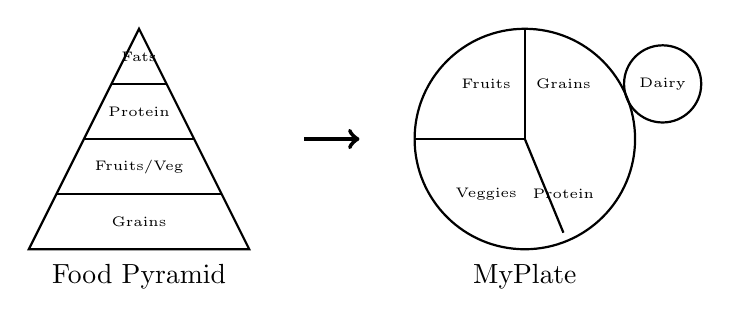
\begin{tikzpicture}[scale=0.7]
				% Old pyramid
				\draw[thick] (0,0) -- (2,4) -- (4,0) -- cycle;
				\draw[thick] (0.5,1) -- (3.5,1);
				\draw[thick] (1,2) -- (3,2);
				\draw[thick] (1.5,3) -- (2.5,3);
				\node at (2,0.5) {\tiny Grains};
				\node at (2,1.5) {\tiny Fruits/Veg};
				\node at (2,2.5) {\tiny Protein};
				\node at (2,3.5) {\tiny Fats};
				\node at (2,-0.5) {Food Pyramid};
				
				% Arrow
				\draw[->, ultra thick] (5,2) -- (6,2);
				
				% New plate
				\draw[thick] (9,2) circle (2cm);
				\draw[thick] (9,2) -- (9,4);
				\draw[thick] (9,2) -- (7,2);
				\draw[thick] (9,2) -- (9.7,0.3);
				\node at (8.3,3) {\tiny Fruits};
				\node at (9.7,3) {\tiny Grains};
				\node at (8.3,1) {\tiny Veggies};
				\node at (9.7,1) {\tiny Protein};
				\draw[thick] (11.5,3) circle (0.7cm);
				\node at (11.5,3) {\tiny Dairy};
				\node at (9,-0.5) {MyPlate};
			\end{tikzpicture}
		\end{center}
	\end{frame}
	
	\begin{frame}{Stereotypes as Flawed Models: The Danger of Over-Simplification}
		\begin{itemize}
			\item \textbf{Stereotypes} are mental models that assume all members of a group share certain characteristics—they're the lazy person's abstraction.
			\item While our brains naturally categorize to handle information efficiently, stereotypes fail because they ignore individual differences and complexity.
			\item These flawed models can lead to discrimination, missed opportunities, and self-fulfilling prophecies when people are treated according to the stereotype.
			\item The key difference between useful models and harmful stereotypes is that good models update with new information, while stereotypes resist change.
		\end{itemize}
		
		\begin{alertblock}{Critical Thinking Check}
			\scriptsize
			When you catch yourself thinking "All X people are Y," you're using a stereotype model. Ask yourself: What evidence supports this? What examples contradict it? Am I missing important individual differences?
		\end{alertblock}
	\end{frame}
	
	\begin{frame}{Scientific Models: From Hypothesis to Theory}
		\begin{itemize}
			\item Scientific models begin as \textbf{hypotheses}—educated guesses about how something works based on initial observations.
			\item Scientists test these models through experiments, looking for evidence that supports or contradicts their predictions.
			\item Models that consistently match experimental results and make accurate predictions may become \textbf{theories}—our best current explanations.
			\item Even well-established theories remain models that could be replaced if new evidence shows they're incomplete or wrong.
		\end{itemize}
		
		\begin{block}{The Scientific Model Cycle}
			\begin{center}
				Observation → Hypothesis → Prediction → Experiment → \\
				Revision → Better Model → More Testing → Theory
			\end{center}
			This cycle never truly ends—even our best theories are still models subject to revision.
		\end{block}
	\end{frame}
	
	\begin{frame}{The Solar System Model: Textbooks vs. Reality}
		\begin{itemize}
			\item Textbook diagrams show planets in neat circular orbits around the sun, all conveniently fitting on one page.
			\item These models grossly distort both \textbf{scale and distance}—if Earth were a pea, Jupiter would be 1000 feet away and the sun would be a beach ball.
			\item The orbits aren't circles but ellipses, planets don't orbit in the same plane, and the sun itself wobbles as planets pull on it.
			\item Despite these "lies," the simplified model successfully teaches the basic concept of planetary motion better than accurate scale would.
		\end{itemize}
		
		
		\begin{table}
			\centering
			\small
			\begin{tabular}{lcc}
				\toprule
				What Textbooks Show & Reality \\
				\midrule
				Circular orbits & Elliptical orbits \\
				Equal spacing & Vast empty distances \\
				Same orbital plane & Tilted at various angles \\
				Stationary sun & Sun orbits galactic center \\
				Planets visible size & Planets are tiny dots \\
				\bottomrule
			\end{tabular}
		\end{table}
	\end{frame}
	
	\begin{frame}
		\frametitle{The Solar System: Scale Model}
		\begin{figure}
			\centering
			% space for the caption or other content.
			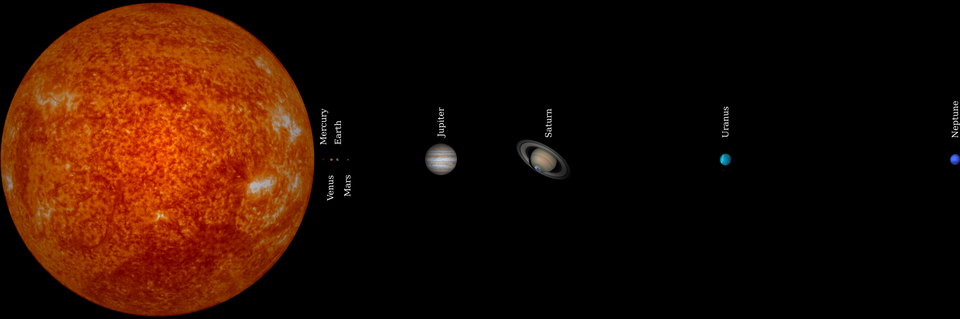
\includegraphics[width=\textwidth, height=0.8\textheight, keepaspectratio]{images/Solar-system.png}
			\small
			\caption{Earth is barely visible!.}
		\end{figure}
	\end{frame}
	
	
	\begin{frame}{Choosing the Right Level of Detail: The Goldilocks Problem}
		\begin{itemize}
			\item Creating useful models requires finding the \textbf{Goldilocks zone}—not too simple, not too complex, but just right for the purpose.
			\item A model with too little detail fails to capture important behavior, while too much detail makes it unwieldy and hard to understand.
			\item The "right" level depends entirely on what you're trying to accomplish—a pilot needs a different weather model than someone planning a picnic.
			\item This judgment improves with experience as you learn which details matter for different purposes and which can safely be ignored.
		\end{itemize}
		
		\begin{example}
			\scriptsize
			Modeling a School Day:
			\begin{itemize}
				\item Too simple: "I go to school" (misses all useful detail)
				\item Just right: Seven periods, lunch, passing time (captures structure)
				\item Too complex: Every conversation, step, and thought (overwhelming)
				\item Purpose matters: Add detail for scheduling, remove it for explaining to grandparents
			\end{itemize}
		\end{example}
	\end{frame}
	
	\begin{frame}{When Models Break: Recognizing Limitations}
		\begin{itemize}
			\item Every model has \textbf{boundary conditions}—situations where it stops working because assumptions no longer hold true.
			\item Newton's laws of motion work perfectly for everyday speeds but break down as objects approach the speed of light, requiring Einstein's relativity.
			\item Economic models failed to predict the 2008 financial crisis because they didn't account for widespread irrational behavior and systemic risks.
			\item Recognizing when you're pushing a model beyond its limits is a crucial skill that prevents dangerous overconfidence in predictions.
		\end{itemize}
		
		\begin{alertblock}{Warning Signs of Model Failure}
			\begin{itemize}
				\item Predictions become wildly inaccurate
				\item Small changes cause huge differences in outcomes  
				\item The model requires increasingly complex "fixes"
				\item Real-world behavior contradicts basic assumptions
			\end{itemize}
		\end{alertblock}
	\end{frame}
	
	\begin{frame}{Mathematical Models: Equations as Abstractions}
		\begin{itemize}
			\item \textbf{Mathematical models} use equations to represent relationships between different quantities in the real world.
			\item The equation $d = rt$ (distance equals rate times time) models motion by ignoring everything except speed, time, and distance traveled.
			\item These models are powerful because math allows us to manipulate symbols instead of dealing with messy reality directly.
			\item Mathematical models can make precise predictions, but their accuracy depends entirely on whether the simplifying assumptions match the situation.
		\end{itemize}
		
		\begin{block}{From Reality to Equation}
			\begin{center}
				Real situation → Identify key variables → \\
				Assume relationships → Write equation → \\
				Solve mathematically → Interpret results
			\end{center}
			Each step involves choices about what to include and what to ignore.
		\end{block}
	\end{frame}
	
	\begin{frame}{The Ideal Gas Law: When Molecules Don't Interact}
		\begin{itemize}
			\item The \textbf{ideal gas law} ($PV = nRT$) models gas behavior by assuming molecules are point particles that don't interact with each other.
			\item Real gas molecules have volume and attract or repel each other, but these complications often don't matter much at normal conditions.
			\item At high pressure or low temperature, real gases deviate significantly from the ideal model because molecules are squeezed together.
			\item Scientists created more complex models (like van der Waals equation) that add back some reality when the simple model isn't accurate enough.
		\end{itemize}
		
		\begin{center}
			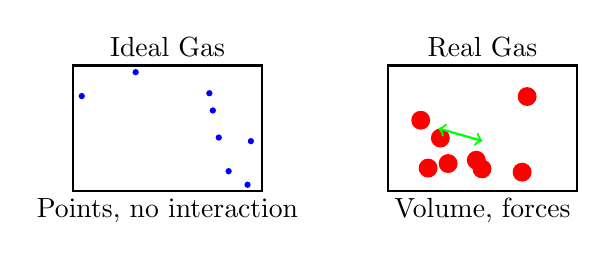
\begin{tikzpicture}[scale=0.8]
				% Ideal gas box
				\draw[thick] (0,0) rectangle (3,2);
				\node at (1.5,2.3) {Ideal Gas};
				\foreach \i in {1,...,8}
				\fill[blue] ({random()*2.8+0.1},{random()*1.8+0.1}) circle (0.05);
				\node at (1.5,-0.3) {Points, no interaction};
				
				% Real gas box  
				\draw[thick] (5,0) rectangle (8,2);
				\node at (6.5,2.3) {Real Gas};
				\foreach \i in {1,...,8} {
					\fill[red] ({random()*2.3+5.3},{random()*1.5+0.25}) circle (0.15);
				}
				\draw[<->, green, thick] (5.8,1) -- (6.5,0.8);
				\node at (6.5,-0.3) {Volume, forces};
			\end{tikzpicture}
		\end{center}
	\end{frame}
	
	\begin{frame}{Personality Models: Myers-Briggs and Beyond}
		\begin{itemize}
			\item Personality models like \textbf{Myers-Briggs} try to categorize the infinite variety of human personalities into a manageable number of types.
			\item These models can provide useful vocabulary for discussing personality differences and help people understand their own tendencies.
			\item However, human personality is far more complex and fluid than any model suggests—people behave differently in different contexts.
			\item The danger comes when we treat these models as fixed truths rather than useful simplifications for specific purposes like team building.
		\end{itemize}
		
		\begin{example}
			Popular Personality Models:
			\begin{itemize}
				\item Myers-Briggs: 16 types based on 4 dimensions
				\item Big Five: Rates 5 traits on continuous scales
				\item Enneagram: 9 interconnected personality types
				\item Each captures some truth but misses individual complexity
			\end{itemize}
		\end{example}
	\end{frame}
	
	\begin{frame}{Computer Simulations: Digital Models of Reality}
		\begin{itemize}
			\item \textbf{Computer simulations} are models that use computational power to track many interacting parts over time.
			\item Flight simulators model aircraft physics, weather, and pilot controls to train pilots without risk or expense of real flying.
			\item Climate models divide Earth into millions of grid cells and simulate decades of weather to predict long-term changes.
			\item These digital models can include more complexity than paper-and-pencil models, but they still require simplifying assumptions about what matters.
		\end{itemize}
		
		\begin{table}
			\centering
			\small
			\begin{tabular}{lll}
				\toprule
				Simulation Type & Models & Ignores \\
				\midrule
				Flight simulator & Aerodynamics, controls & Bird strikes, wear \\
				Climate model & Ocean, atmosphere & Individual clouds \\
				Traffic simulation & Driver behavior & Radio stations \\
				Disease spread & Contact patterns & Individual immunity \\
				\bottomrule
			\end{tabular}
		\end{table}
	\end{frame}
	
	\begin{frame}{The Spherical Cow: A Classic Physics Joke About Over-Idealization}
		\begin{itemize}
			\item Physicists joke about modeling a cow as a \textbf{sphere} to illustrate how scientific models can become absurdly oversimplified.
			\item The joke originated from physics problems that begin "Assume a spherical cow in a vacuum..." to eliminate messy biological reality.
			\item While it sounds ridiculous, spherical cow models can actually work for some calculations, like estimating how much hay a herd needs.
			\item The joke reminds us to always ask whether our simplifications have gone too far for the problem we're trying to solve.
		\end{itemize}
		
		\begin{center}
			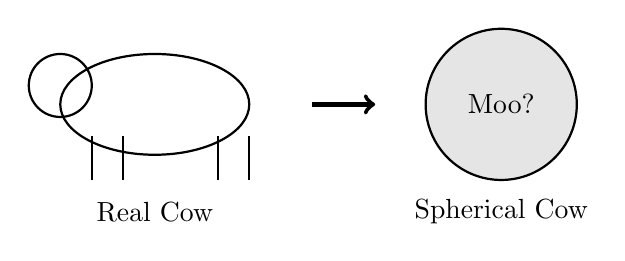
\begin{tikzpicture}[scale=0.8]
				% Real cow (simplified)
				\draw[thick] (-2,0) ellipse (1.5cm and 0.8cm);
				\draw[thick] (-3.5,0.3) circle (0.5cm);
				\draw[thick] (-0.5,-0.5) -- (-0.5,-1.2);
				\draw[thick] (-1,-0.5) -- (-1,-1.2);
				\draw[thick] (-2.5,-0.5) -- (-2.5,-1.2);
				\draw[thick] (-3,-0.5) -- (-3,-1.2);
				\node at (-2,-1.7) {Real Cow};
				
				% Arrow
				\draw[->, ultra thick] (0.5,0) -- (1.5,0);
				
				% Spherical cow
				\draw[thick, fill=black!10] (3.5,0) circle (1.2cm);
				\node at (3.5,-1.7) {Spherical Cow};
				\node at (3.5,0) {Moo?};
			\end{tikzpicture}
		\end{center}
	\end{frame}
	
	\begin{frame}{Models in Medicine: From Anatomy Diagrams to Disease Spread}
		\begin{itemize}
			\item Medical models range from \textbf{anatomical diagrams} that show body structure to epidemiological models that predict disease spread.
			\item The classic heart diagram shows four chambers and major vessels but ignores the electrical system, individual variation, and surrounding tissues.
			\item Disease spread models like SIR (Susceptible-Infected-Recovered) help predict pandemic behavior but assume uniform mixing of populations.
			\item Medical professionals must constantly balance simplified teaching models with the complex reality of individual patient cases.
		\end{itemize}
		
		\begin{block}{The SIR Model}
			\begin{center}
				Susceptible → Infected → Recovered \\
				\vspace{0.2cm}
				This simple flow model helped predict COVID-19 spread, despite ignoring factors like asymptomatic cases, varying immunity, and behavior changes.
			\end{center}
		\end{block}
	\end{frame}
	
	\begin{frame}{Time Management Models: Calendars and Schedules}
		\begin{itemize}
			\item \textbf{Calendars and schedules} are models that represent the continuous flow of time as discrete blocks we can manipulate and plan.
			\item These models assume tasks fit neatly into time slots, but reality includes interruptions, transitions, and tasks that expand or contract.
			\item Different calendar models work for different people—some need hourly detail while others work better with flexible daily goals.
			\item The most common failure is creating an "ideal day" model that ignores how much time real activities actually take.
		\end{itemize}
		
		\begin{example}
			Time Model vs. Reality:
			\begin{itemize}
				\item Schedule says: Math homework 7:00-8:00 PM
				\item Reality includes: Finding materials (10 min), mental transition (5 min), checking phone (15 min), actual work (45 min), cleanup (5 min)
				\item Effective models build in buffer time for reality
			\end{itemize}
		\end{example}
	\end{frame}
	
	\begin{frame}{Building Good Models: Key Questions to Ask}
		\begin{itemize}
			\item Before creating any model, ask \textbf{"What is my purpose?"}—a model for understanding differs from one for prediction or communication.
			\item Identify the essential features by asking \textbf{"What must I include?"}—these are the elements without which the model fails completely.
			\item Consider your audience with \textbf{"Who will use this model?"}—experts can handle more complexity than beginners.
			\item Finally, ask \textbf{"How will I know if it works?"}—good models have clear criteria for success or failure.
		\end{itemize}
		
		\begin{block}{The Model Builder's Checklist}
			\scriptsize
			\begin{enumerate}
				\item Define clear purpose and scope
				\item List assumptions explicitly  
				\item Identify key variables and relationships
				\item Choose appropriate level of detail
				\item Plan how to test the model
				\item Consider when the model might fail
			\end{enumerate}
		\end{block}
	\end{frame}
	
	\begin{frame}{Testing Models: Prediction vs. Reality}
		\begin{itemize}
			\item The ultimate test of any model is whether its \textbf{predictions match reality} within acceptable error bounds.
			\item Good models make specific, testable predictions—vague models that can explain anything actually explain nothing.
			\item When predictions fail, it reveals either wrong assumptions, missing variables, or situations beyond the model's scope.
			\item Testing should include both typical cases where the model should work and edge cases where it might break down.
		\end{itemize}
		
		\begin{example}
			\scriptsize
			Testing a Study Time Model:
			\begin{itemize}
				\item Model predicts: 2 hours study = B grade, 3 hours = A grade
				\item Test with real data: Track actual study time and grades
				\item Discover complications: Subject difficulty matters, quality beats quantity, some students need more time
				\item Refine model: Add subject difficulty multiplier and efficiency factors
			\end{itemize}
		\end{example}
	\end{frame}
	
	\begin{frame}{Multiple Models: Why Different Views Matter}
		\begin{itemize}
			\item Complex phenomena often require \textbf{multiple models} that each capture different aspects of reality.
			\item Light behaves as both a wave and a particle—physicists use whichever model works better for each situation.
			\item In business, financial models show profitability while organizational models show human relationships—both are needed for success.
			\item Using multiple models helps avoid the tunnel vision that comes from relying on a single perspective.
		\end{itemize}
		
		\begin{center}
			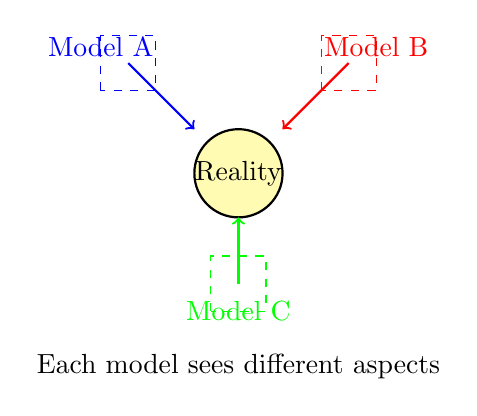
\begin{tikzpicture}[scale=0.7]
				% Center object
				\draw[thick, fill=yellow!30] (0,0) circle (0.8cm);
				\node at (0,0) {Reality};
				
				% Different model views
				\draw[thick, ->, blue] (-2,2) -- (-0.8,0.8);
				\node[blue] at (-2.5,2.3) {Model A};
				\draw[blue, dashed] (-2.5,1.5) rectangle (-1.5,2.5);
				
				\draw[thick, ->, red] (2,2) -- (0.8,0.8);
				\node[red] at (2.5,2.3) {Model B};
				\draw[red, dashed] (1.5,1.5) rectangle (2.5,2.5);
				
				\draw[thick, ->, green] (0,-2) -- (0,-0.8);
				\node[green] at (0,-2.5) {Model C};
				\draw[green, dashed] (-0.5,-2.5) rectangle (0.5,-1.5);
				
				\node at (0,-3.5) {Each model sees different aspects};
			\end{tikzpicture}
		\end{center}
	\end{frame}
	
	\begin{frame}{The Map-Territory Relationship: Models Are Not Reality}
		\begin{itemize}
			\item Philosopher Alfred Korzybski famously said \textbf{"The map is not the territory"}—models represent reality but are not reality itself.
			\item It's easy to forget this distinction and start believing our models are more real than the messy world they represent.
			\item This confusion leads to problems like treating IQ scores as complete measures of intelligence or GDP as the sole measure of national success.
			\item Always remember that models are tools for thinking about reality, not substitutes for experiencing and observing the real world.
		\end{itemize}
		
		\begin{alertblock}{The Fundamental Warning}
			No matter how detailed, accurate, or useful a model becomes, it remains a simplified representation. The moment you forget this and mistake the model for reality itself, you've fallen into one of thinking's most dangerous traps.
		\end{alertblock}
	\end{frame}
	
	
\begin{frame}{Models in Decision Making: Pros and Cons Lists}
	\begin{itemize}
		\item The humble \textbf{pros and cons list} is actually a decision-making model that simplifies complex choices into positive and negative factors.
		\item This model assumes all factors can be clearly categorized and that more items on one side means that choice is better.
		\item Advanced versions assign weights to different factors, recognizing that not all pros and cons matter equally.
		\item The model's simplicity is both its strength (easy to use) and weakness (ignores factor interactions and emotional elements).
	\end{itemize}
	
	\begin{table}
		\centering
		\small
		\begin{tabular}{ll|ll}
			\multicolumn{2}{c|}{Simple Model} & \multicolumn{2}{c}{Weighted Model} \\
			\hline
			Pros & Cons & Pros (Weight) & Cons (Weight) \\
			\hline
			Closer & Expensive & Closer (3) & Expensive (5) \\
			Better teachers & Less diverse & Better teachers (4) & Less diverse (2) \\
			Nice campus & Far from home & Nice campus (1) & Far from home (3) \\
			\hline
			Count: 3 & Count: 3 & Score: 8 & Score: 10 \\
		\end{tabular}
	\end{table}
\end{frame}

\begin{frame}{Evolution of Models: How Our Understanding Improves}
	\begin{itemize}
		\item Models evolve through a process of \textbf{iterative refinement}—each version builds on lessons learned from previous failures.
		\item Early models tend to be simple and capture only the most obvious features, like ancient astronomers tracking basic star movements.
		\item As we gather more data and identify model failures, we add complexity where needed while trying to maintain usability.
		\item Sometimes incremental improvements aren't enough, and we need \textbf{paradigm shifts}—completely new models that approach problems differently.
	\end{itemize}
	
	\begin{block}{Model Evolution Pattern}
		\begin{center}
			Simple observation → Basic model → Find exceptions → \\
			Add complexity → Test again → Reach limits → \\
			Revolutionary new approach → Repeat cycle
		\end{center}
		This pattern appears across all fields from physics to psychology.
	\end{block}
\end{frame}

\begin{frame}{The Cost of Complexity: When Simple Models Work Better}
	\begin{itemize}
		\item Adding detail to models has \textbf{diminishing returns}—each new factor makes the model harder to use while providing less additional accuracy.
		\item Complex models require more data, more computation, and more expertise to use effectively than simple ones.
		\item In many situations, a simple model that's "good enough" beats a complex model that's theoretically better but practically unwieldy.
		\item The art lies in finding the sweet spot where additional complexity stops adding value for your specific purpose.
	\end{itemize}
	
	\begin{center}
		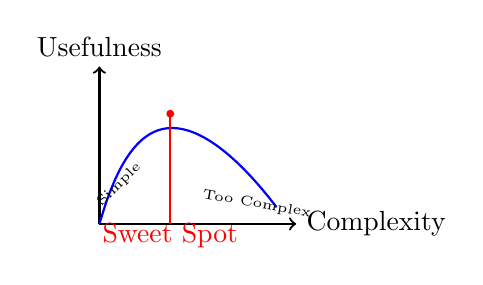
\begin{tikzpicture}[scale=0.5]
			% Axes
			\draw[thick,->] (0,0) -- (5,0) node[right] {Complexity};
			\draw[thick,->] (0,0) -- (0,4) node[above] {Usefulness};
			
			% Curve showing diminishing returns
			\draw[thick,blue] plot[smooth,domain=0:4.5] (\x,{3.5*(1-exp(-\x))-0.15*\x*\x});
			
			% Sweet spot
			\fill[red] (1.8,2.8) circle (0.1);
			\draw[red,thick] (1.8,0) -- (1.8,2.8);
			\node[red] at (1.8,-0.3) {Sweet Spot};
			
			% Labels
			\node at (0.5,1) [rotate=45] {\tiny Simple};
			\node at (4,0.5) [rotate=-10] {\tiny Too Complex};
		\end{tikzpicture}
	\end{center}
\end{frame}

\begin{frame}{Thinking Like a Modeler: Applying These Tools to Your Life}
	\begin{itemize}
		\item Recognizing models everywhere helps you think more clearly about \textbf{what assumptions you're making} in daily life.
		\item When facing problems, ask "What would a useful model of this situation include?" to identify key factors and relationships.
		\item Practice building multiple models of the same situation to avoid getting locked into one perspective or solution.
		\item Most importantly, stay humble about your models—be ready to revise or abandon them when reality proves them inadequate.
	\end{itemize}
	
	\begin{example}
		\scriptsize
		Modeling Your Day Tomorrow:
		\begin{itemize}
			\item Energy model: When will I have high/low energy for different tasks?
			\item Time model: How long will activities actually take (with buffers)?
			\item Social model: Who will I interact with and how will that affect plans?
			\item Combine insights from all three for a realistic, flexible plan
		\end{itemize}
	\end{example}

\end{frame}

\end{document}